\documentclass[12pt,titlepage,a4page , tikz , multi,table , svgnames,xcdraw]{article}
\usepackage{graphicx}
\usepackage[svgnames , table , xcdraw]{xcolor} 
\usepackage{fancyhdr}
 
\usepackage{hyperref}
\hypersetup{
    colorlinks=true,
    linkcolor=blue,
    filecolor=magenta,      
    urlcolor=cyan,
}

\usepackage{mathtools}
\usepackage{multirow}
\usepackage{graphicx}
\usepackage{float}
\usepackage{enumitem}
\usepackage{listings }
\usepackage[a4paper, total={6in, 8in}]{geometry}
\usepackage{afterpage}
\usepackage{amssymb}
\usepackage{pdflscape}
\usepackage{lscape}
\usepackage{amsmath}
\usepackage{svg}
\usepackage[final]{pdfpages}

\usepackage{pgf, tikz}
\usetikzlibrary{arrows, automata}
\usetikzlibrary{shapes.multipart}


\usepackage[T1]{fontenc}
\usepackage{tikz}
\usepackage[utf8]{inputenc} % Required for inputting international characters
\usepackage{PTSerif} 

\usepackage{float}

\usepackage[Kashida]{xepersian}
\settextfont[
 BoldFont={XB NiloofarBd.ttf}
 ]{XB Niloofar.ttf}


\NewDocumentCommand{\codeword}{v}{
\texttt{\textcolor{blue}{#1}}
}
\DeclareFixedFont{\ttb}{T1}{txtt}{bx}{n}{12} % for bold
\DeclareFixedFont{\ttm}{T1}{txtt}{m}{n}{12}  % for normal


\definecolor{deepblue}{rgb}{0,0,0.5}
\definecolor{deepred}{rgb}{0.6,0,0}
\definecolor{deepgreen}{rgb}{0,0.5,0}

\newcommand\independent{\protect\mathpalette{\protect\independenT}{\perp}}
\def\independenT#1#2{\mathrel{\rlap{$#1#2$}\mkern2mu{#1#2}}}

% Python style for highlighting
\newcommand\pythonstyle{\lstset{
language=Python,
basicstyle=\ttm,
otherkeywords={self},             % Add keywords here
keywordstyle=\ttb\color{deepblue},
emph={MyClass,__init__},          % Custom highlighting
emphstyle=\ttb\color{deepred},    % Custom highlighting style
stringstyle=\color{deepgreen},
frame=tb,                         % Any extra options here
showstringspaces=false            % 
}}


% Python environment
\lstnewenvironment{python}[1][]
{
\pythonstyle
\lstset{#1}
}
{}

% Python for external files
\newcommand\pythonexternal[2][]{{
\pythonstyle
\lstinputlisting[#1]{#2}}}

\newenvironment{changemargin}[2]{%
\begin{list}{}{%
\setlength{\topsep}{0pt}%
\setlength{\leftmargin}{#1}%
\setlength{\rightmargin}{#2}%
\setlength{\listparindent}{\parindent}%
\setlength{\itemindent}{\parindent}%
\setlength{\parsep}{\parskip}%
}%
\item[]}{\end{list}}

% Python for inline
\newcommand\pythoninline[1]{{\pythonstyle\lstinline!#1!}}


\begin{document}

\begin{titlepage}

 \begin{center}
        
       \vspace*{1cm}

 \vspace{1cm}
       \textbf{ \Huge{به نام خدا} }
       \vspace{0.4cm}
       
       \includegraphics[width=0.4\textwidth]{sharif1.png}
       
 	\vspace{0.7cm}
       \textbf{ \LARGE{معماری کامپیوتر} }

 
   \vspace{0.7cm}
  \textbf{ \Large{ پروژه پایانی - بخش اول - طراحی پردازنده} }
   \vspace{0.5cm}
       
 
      \large \textbf{دانشکده مهندسی کامپیوتر}\\\vspace{0.2cm}
    \large   دانشگاه صنعتی شریف\\\vspace{0.25cm}
      
استاد:\\
    \textbf{{جناب آقای دکتر اسدی}}

    \vspace{0.15cm}
    \noindent\rule[1ex]{\linewidth}{3pt}
    
    \vspace{0.5cm}
نام و نام خانوادگی اعضای گروه:\\
    \textbf{{سپهر پورقناد - 97101359}}
        \vspace{0.1cm}
        
     \textbf{{سیدمحمدصادق کشاورزی - 97106249}}
        \vspace{0.1cm}
        
       \textbf{{امیرمهدی نامجو - 97107212}}
        \vspace{0.1cm}


\end{center}
\end{titlepage}

\newpage
\pagestyle{fancy}
\fancyhf{}
\fancyfoot{}

\cfoot{\thepage}
\chead{پروژه پایانی}
\rhead{طراحی پردازنده}
\lhead{معماری کامپیوتر}



\newpage

\section{مقدمه}

هدف اصلی ما در این پروژه، طراحی یک پردازنده ساده براساس دستورات داده شده در مستندات آن و تست کردن آن به شکلی بوده است که حالات مختلف آن پوشش داده شود. در طراحی پردازنده داده شده، ما از اصول کلی که در درس آموخته ایم و عموما براساس پردازنده مبتنی بر MIPS بوده اند، استفاده کرده ایم. البته در این جا ساختار کلی ما از لحاظ کلی ساده تر از MIPS است. در ادامه گزارش، به توضیح نحوه طراحی بخش های مختلف این پردازنده می پردازیم.

\newpage

\section{طراحی ALU}

بخش ALU در اصل سیستم محاسبه گر اصلی ما است و از آن جایی که بیش تر دستورات داده شده در مستندات پروژه برای اجرای به آن وابستگی دارند، از اهمیت بالایی برخوردار است. برای طراحی ALU به این شکل عمل کرده ایم پنچ ورودی برای آن در نظر گرفته ایم که شامل داده ورودی 1، داده ورودی 2 هر دو به صورت 32 بیتی، مقدار شیفت به صورت 5 بیتی، مقدار cin یعنی carry ورودی به صورت 1 بیتی و همچنین Opcode به صورت چهاربیتی بوده است. 

برای عملیات های مختلف آن، از ماژول هایی که در Quartus در اختیار ما قرار گرفته است، استفاده کرده ایم. برای جمع از ماژول جمع کننده استفاده کرده و همچنین از آن جایی که کوارتوس برای آن از سیستم محاسبه Overflow هم پشتیبانی می کند، آن را هم قرار داده ایم. برای تفریق از ماژول تفریق گر استفاده کرده ایم، البته روش های دیگری هم نظیر نقیض کردن ورودی دوم و استفاده از cin=1 به عنوان ورودی جمع کننده هم برای این کار وجود داشت ولی برای طراحی ساده تر و امکان دیباگ راحت تر، ترجیح دادیم که از ماژول جداگانه استفاده کنیم. برای شیفت به چپ و راست، ماژول های مربوط به آن ها را قرار داده ایم. این ماژول ها مقدار ShiftAmount را با نام distance و خود داده را هم با عنوان data به عنوان ورودی می گیرند. برای NAND یک گیت NAND دو ورودی قرار داده ایم که به ورودی های آنان، با توجه به این که کوارتوس توانایی تشخیص این که از مقادیر چند بیتی استفاده بکنیم را هم دارد، مقادیر 32 بیتی مربوطه را داده و مقدار 32 بیتی خروجی گرفته ایم. برای عملیات \lr{set on less than} از یک ماژول Comparator استفاده کرده ایم. این ماژول به عنوان ورودی دو داده 32 بیتی را گرفته و در خروجی دو داده به ما می دهد؛ داده aeb در صورتی که $1$ باشد، بیانگر برابر بودن دو مقدار و در غیر این صورت، بیانگر نامساوی بودن آنان است، داده alb هم در صورت یک بودن، نشانگر کوچکتر بودن a از b و در غیر این صورت نشان دهنده بزرگتر مساوی بودن b از a است. از سیگنال alb برای حالت slt استفاده کرده ایم و از آن جایی که این خروجی 1 بیتی است ولی به عنوان خروجی ALU ما 32 بیت می خواهیم، سایر بیت ها را از طریق اتصال به GND صفر کردیم. در نهایت هم ماژول min را استفاده کرده ایم که همان طور که از نامش مشخص است، کمینه دو داده را حساب می کند.

برای انتخاب این که خروجی کدام ماژول باید به عنوان خروجی نهایی داده شود، از یک مالتی پلکسر 32 بیتی 8 به 1 استفاده کرده ایم که البته حالت $100$ آن استفاده خاصی ندارد. برای خروجی sgn که نشانگر علامت خروجی است، از بیت $31$ مقدار خروجی این مالتی پلکسر استفاده کرده ایم. همچنین برای خروجی eq هم از خروجی aeb ماژول Comparator استفاده کرده ایم. برای Overflow هم از آن جایی که سوال گفته فقط برای جمع باید در نظر گرفته شود، گیت هایی قرار داده ایم که براساس OpCode تنها درصورتی که در حالت جمع باشیم، مقدار Overflow ماژول جمع کننده به خروجی برود و در غیر این صورت، $0$ به خروجی برود. یک ماژول به اسم zero هم قرار داده ایم که در اصل در پیاده سازی داخلی همان comparator است با این تفاوت که یکی از داده های آن به شکل درونی صفر شده است و مشخص می کند که آیا خروجی نهایی برابر صفر است یا نه.

شکل کلی ماژول ALU در صفحه بعد قرار دارد.



\begin{landscape}

\thispagestyle{empty}

\includepdf[pages=1,angle=90, ]{ALU.pdf}


\end{landscape}




\section{طراحی واحد کنترل}

برای طراحی این پردازنده، ما از 4 کلاک استفاده کرده ایم که در شکل زیر \lr{State Machine} آن قرار گرفته است.



\begin{center}


\begin{latin}
    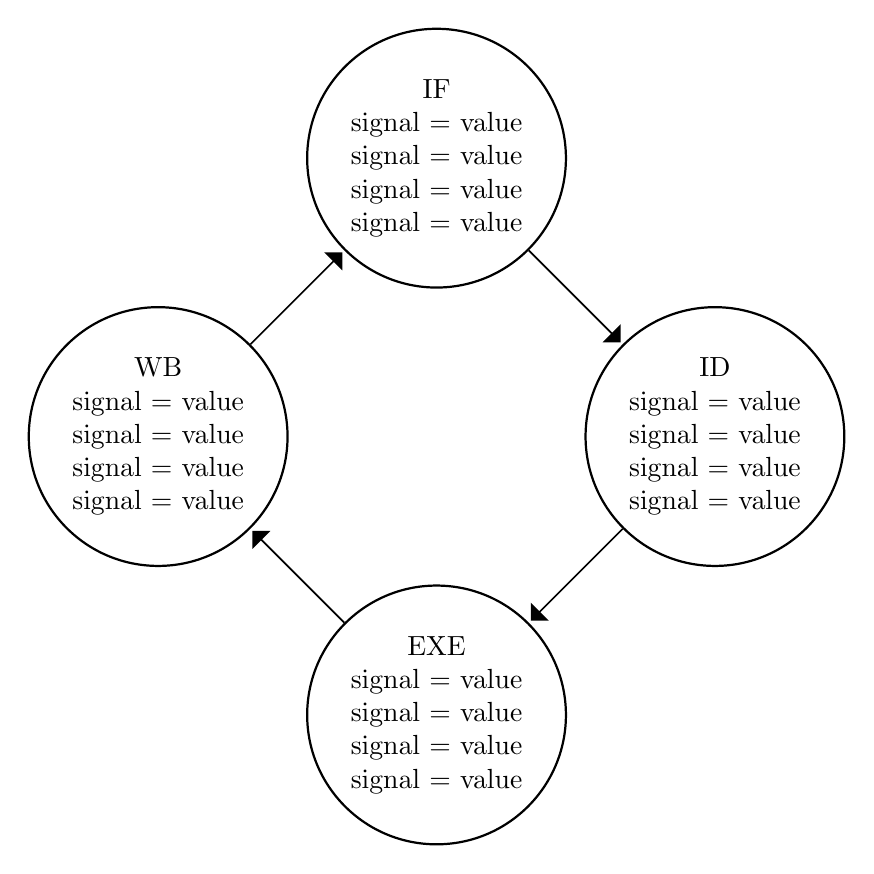
\begin{tikzpicture}[
            > = triangle 90, % arrow head style
            shorten > = 1pt, % don't touch arrow head to node
            auto 
            ,
            node distance = 5cm, % distance between nodes
            semithick
            , every text node part/.style={align=center} % line style
        ]

        \tikzstyle{every state}=[
            draw = black,
            thick,
            fill = white,
            minimum size = 4mm
        ]
		
        \node[state] (IF) [] {IF  \\ signal = value \\ signal = value \\ signal = value \\ signal = value};
        \node[state] (ID) [below right of=IF] {ID \\ signal = value \\ signal = value \\ signal = value \\ signal = value};
        \node[state] (EXE) [below left of=ID ] {EXE  \\ signal = value \\ signal = value \\ signal = value \\ signal = value};
        \node[state] (WB) [above left of=EXE] {WB  \\ signal = value \\ signal = value \\ signal = value \\ signal = value};
  






        
		\path[->] (IF) edge node {} (ID);
		\path[->] (ID) edge node {} (EXE);
		\path[->] (EXE) edge node {} (WB);
		\path[->] (WB) edge node {} (IF);
		
       
    \end{tikzpicture}

\end{latin}
\end{center}


شکل واحد کنترل در صفحه بعد قرار دارد.

\begin{landscape}

\thispagestyle{empty}

\includepdf[pages=1,angle=90, ]{CU.pdf}


\end{landscape}




\newpage

\section{مقداردهی حافظه دستورات}

برای حافظه دستورات ما از بخش \lr{Mega-Plugin Wizard} ارائه شده توسط Quartus و مقدار دهی ROM براساس فایل mif مشابه راهنمای قرار گرفته در مستند پروژه استفاده کرده ایم. یکی از نکات قابل توجه این جاست که در CycloneII که تا به حال طراحی های کوارتوس را با آن انجام دادیم، نمی توان رام چندان بزرگی استفاده کرد و مجبور شدیم از رامی با اندازه 32768 کلمه 20 بیتی استفاده کنیم و برای تعداد کلمه بزرگ تر، در هنگام کامپایل به خطای در اختیار نبودن منبع برای سنتز چنین چیزی روی CycloneII بر می خوردیم.

محتویات فایل mif قرار گرفته بدین صورت است. در جلوی دستورات به صورت کامنت، کاری که دستور انجام می دهد هم مشخص شده است:

\begin{latin}
\begin{verbatim}
WIDTH=20;
DEPTH=32768;
ADDRESS_RADIX = UNS;          -- The radix for address values is unsigned
DATA_RADIX = BIN;             -- The radix for data values is Binary
CONTENT                       -- start of (address : data pairs)
BEGIN
0 : 10000000000000100001; -- load shamt r1 <-1
1 : 10000000000000100010; -- load shamt r2 <-1
2 : 10000000000001000011; -- load shamt r3 <-10
3 : 10000000000010000100; -- load shamt r4 <-100
4 : 00110000011111000001; -- r1 = r1 << 30
5 : 00000000000000100001; -- r1 = r0 + r1 (0)
6 : 00000000000001000010; -- r2 = r0 + r2 (0)
7 : 00000000000001100011; -- r3 = r0 + r3 (0)
8 : 00000000000010000100; -- r4 = r0 + r4 (0)
9 : 00000000100001000101; -- r5 = r2 + r2
10 : 00000000010000100110; -- r6 = r1 + r1  -> must overflow
11 : 00100001000000100100; -- r4 = r4 >> 1
12 : 01010001000001100111; -- r7 = r4 ~& r3
13 : 01110000000010001000; -- r8 = set on less than (r0 , r4)
14 : 01100000100010001001; -- r9 = min(r2 , r4)
15 : 10000000000000101010; -- load shamt r10 <-1
16 : 00001000000101001011; -- r11 = r0 - r10 (answer must be -1)
17 : 00000000000000100001; -- r1 = r0 + r1 (0)
18 : 00000000000001000010; -- r2 = r0 + r2 (0)
19 : 00000000000001100011; -- r3 = r0 + r3 (0)
20 : 00000000000001000010; -- r4 = r0 + r4 (0)
21 : 00000000000010100101; -- r5 = r0 + r5 (0)
22 : 00000000000011000110; -- r6 = r0 + r6 (0)
23 : 00000000000011100111; -- r7 = r0 + r7 (0)
24 : 00000000000100001000; -- r8 = r0 + r8 (0)
25 : 00000000000100101001; -- r9 = r0 + r9 (0)
26 : 00001000000101001010; -- r10 = r0 + r10 + cin(1)
27 : 00000000000101101011; -- r11 = r0 + r11
28:  00000000000101001010; -- r10 = r0 + r10
[29..32767] : 00000000000000000000;
END;

\end{verbatim} 
\end{latin}

نکته مهم در مورد دستورات آخر که اکثرا جمع با صفر هستند، این است که به کمک این دستورات و Output های قرار داده شده، مقادیر هر کدام از رجیسترها را مشاهده بکنیم که ببینیم آیا در نهایت مقادیر قرار گرفته در آنان درست است یا نه.

خروجی های نهایی رجیسترها، باید به شکل زیر باشد (یعنی در خط های آخر، باید این اعداد را مشاهده کنیم):

\begin{latin}

\begin{verbatim}

R1 = 1073741824
R2 = 1
R3 = 2
R4 = 1
R5 = 2
R6 = -2147483648 -- this is caused by overflow on address 10
R7 = -3
R8 = 1
R9 = 1
R10 = on line 26 it is 1 and then on address 28 it is 2
R11 = 2



\end{verbatim}


\end{latin}

ضمنا باید توجه کنیم که این ROM ها به صورت Word-Addressable هستند و از طرفی PC ما چهار واحد چهار واحد جلو می رود و همچنین با توجه به فضای داده شده، برای یافتن آدرس درست تنها به 15 بیت نیاز دارند، ما از بیت $2$ تا $16$ PC را به آن به عنوان ورودی آدرس داده ایم. دو بیت اول در اصل همیشه $0$ هستند و با توجه به Word-Addressable بودن رام نیازی به آن نیست.


\newpage



\end{document}












